\documentclass{article}
\usepackage{amsmath}
\usepackage{graphicx} 
\usepackage{xcolor}
\usepackage{listings}
\usepackage{hyperref}
\usepackage{cleveref}
\usepackage{geometry}
\usepackage{enumitem}

% tikz stuff
\usepackage{tikz}
\usepackage{pgfplots}
\usepackage{circuitikz}

% pstricks
\usepackage{pstricks}

\title{Test Title}
\author{Dan Lynch}
\date{v0.0.1 January 2025}

\begin{document}

\maketitle

\tableofcontents

\section{Introduction}

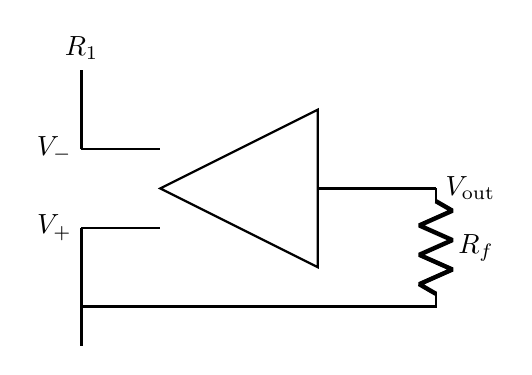
\begin{tikzpicture}
  % Draw the op-amp triangle
  \draw[thick] (0,0) -- (2,1) -- (2,-1) -- cycle;
  
  % Draw and label the inverting input (-)
  \draw[thick] (-1,0.5) -- (0,0.5);
  \node[left] at (-1,0.5) {$V_-$};
  \draw[thick] (-1,0.5) -- (-1,1.5) node[above] {$R_1$};
  
  % Draw and label the non-inverting input (+)
  \draw[thick] (-1,-0.5) -- (0,-0.5);
  \node[left] at (-1,-0.5) {$V_+$};
  
  % Output
  \draw[thick] (2,0) -- (3.5,0);
  \node[right] at (3.5,0) {$V_{\text{out}}$};
  
  % Feedback loop
  \draw[thick] (3.5,0) to[R, l=$R_f$] (3.5,-1.5) -- (-1,-1.5) -- (-1,-0.5);
  
  % Ground for non-inverting input
  \draw[thick] (-1,-1.5) to[ground] (-1,-2);
\end{tikzpicture}

\begin{pspicture}(0,-3)(8,3)
  \rput(0,0){$x(t)$}
  \rput(4,1.5){$f(t)$}
  \rput(4,-1.5){$g(t)$}
  \rput(8.2,0){$y(t)$}
  \rput(1.5,-2){$h(t)$}
  \psframe(1,-2.5)(7,2.5)
  \psframe(3,1)(5,2)
  \psframe(3,-1)(5,-2)
  \rput(4,0){$X_k = \frac{1}{p} \sum \limits_{n=\langle p\rangle}x(n)e^{-ik\omega_0n}$}
  \psline{->}(0.5,0)(1.5,0)
  \psline{->}(1.5,1.5)(3,1.5)
  \psline{->}(1.5,-1.5)(3,-1.5)
  \psline{->}(6.5,1.5)(6.5,0.25)
  \psline{->}(6.5,-1.5)(6.5,-0.25)
  \psline{->}(6.75,0)(7.75,0)
  \psline(1.5,-1.5)(1.5,1.5)
  \psline(5,1.5)(6.5,1.5)
  \psline(5,-1.5)(6.5,-1.5)
  \psline(6,-1.5)(6.5,-1.5)
  \pscircle(6.5,0){0.25}
  \psline(6.25,0)(6.75,0)
  \psline(6.5,0.5)(6.5,-0.5)
  \end{pspicture}

\end{document}